% !TeX program = xelatex
\documentclass[UTF8,a4paper,12pt]{ctexart}
\usepackage{geometry}
\geometry{left=2.5cm,right=2.5cm,top=2.4cm,bottom=2.4cm}
\usepackage{setspace}
\setstretch{1.35}
\usepackage{fancyhdr}
\pagestyle{fancy}
\fancyhf{}
\fancyhead[C]{\small 基于圆拟合中心线的古塔变形分析}
\fancyfoot[C]{\thepage}
\setlength{\headheight}{14pt}
\usepackage{amsmath,amssymb,bm}
\usepackage{booktabs,longtable,array,multirow}
\usepackage{graphicx,float,caption}
\usepackage{hyperref}
\usepackage{xcolor}
\usepackage{enumitem}
\captionsetup[table]{position=top}
\captionsetup[figure]{position=bottom}
\hypersetup{colorlinks=true,linkcolor=black,citecolor=black,urlcolor=blue}
\newcommand{\upcite}[1]{\textsuperscript{\cite{#1}}}
\newcommand{\figpath}{..}
\title{\heiti 基于最小二乘圆拟合与中心线回归的古塔变形分析模型}
\author{}
\date{}

\begin{document}
\maketitle
\thispagestyle{empty}

\begin{abstract}
古塔在长期自重、温度、风荷载和偶然地震作用下会产生倾斜、弯曲与扭曲等综合变形。本文依据1986年、1996年、2009年和2011年四次测量数据，建立了“同层测点圆拟合--相对底层中心线--轴线回归--趋势外推”的建模链，目标是给出各层中心坐标、评价变形形态并判断未来趋势。

针对问题一，本文把每一层外轮廓测点看作近似圆周上的离散观测点，采用代数最小二乘圆拟合确定该层中心；对塔尖多点数据用均值中心处理，对缺测点不作人为插值。计算得到四次测量共55组中心坐标，其中第13层中心相对底层中心偏移量分别为0.6292 m、0.6374 m、0.6791 m和0.6808 m。圆拟合残差中位数为0.0500 m，最大均方根残差为0.0774 m，说明圆截面中心法可稳定提取塔身轴线。

针对问题二，本文以各年度底层中心为局部坐标原点，排除不同时期测量坐标基准平移对变形判断的影响。倾斜分析表明，2011年第13层中心相对底层中心的水平偏移为0.6808 m，倾角为0.7640°，方向角约322.20°，整体向东偏北方向倾斜；弯曲分析采用中心线相对最佳直线轴的水平残差刻画，1986年最大弯曲残差为0.0197 m，2009年和2011年增至约0.0619 m，表明塔身并非单纯刚体倾斜，而存在明显轴线弯曲；扭曲分析用同层标志点相对中心的极角变化度量，各年最大相对扭转约4.02°--5.37°，属于可观测但弱于倾斜和弯曲的变形。

针对问题三，本文对各层相对位移建立线性趋势模型，并用1986--2011年四期数据进行回归。结果显示，第13层偏移量年均增加约2.25 mm，线性拟合的决定系数为0.9454；其中$x$向位移趋势不明显，而$y$向负向位移趋势显著，说明塔顶水平位移增长主要来自北向分量增加。模型预测2021年第13层偏移量约0.7051 m，2030年约0.7286 m，倾斜方向角分别约319.72°和317.55°。

本文进一步进行了基准坐标、圆拟合残差、线性轴残差和趋势外推的稳健性检查。与“直接取测点均值”基线方法相比，圆拟合法能利用圆周几何约束抑制局部测点缺失和噪声；与“只看塔顶偏移”的简单评价相比，中心线回归同时揭示了倾斜、弯曲与扭曲三类变形。模型结构清晰、可复现，但受限于仅四期观测，长期趋势预测仍应结合后续监测滚动修正。

\textbf{关键词：}古塔变形；最小二乘圆拟合；中心线回归；倾斜分析；趋势预测
\end{abstract}

\newpage
\tableofcontents
\newpage

\section{问题重述}
\subsection{问题背景}
古塔是具有重要历史、艺术和工程价值的文物建筑。由于年代久远，塔体长期承受自重、地基沉降、温度变化、风荷载等持续作用，并可能经历地震、飓风等偶然荷载，塔身会逐渐偏离原始几何形态。常见变形包括整体倾斜、局部弯曲、截面扭转以及不同高度上的复合位移。对古塔变形进行定量分析，不仅可以判断当前安全状态，也能为后续加固、限载、监测点布设和预警阈值制定提供依据。

题目给出了某古塔在1986年7月、1996年8月、2009年3月和2011年3月四次测量获得的空间坐标数据。每次测量均记录了不同塔层若干测点的三维坐标，主体塔身各层一般包含8个环向测点，部分年份和层位存在缺测或塔尖观测方式差异。要求基于这些观测数据，提取各层中心位置，并进一步分析古塔倾斜、弯曲、扭曲等变形特征及其发展趋势。

\subsection{问题要求与输出目标}
结合题意，本文将任务分解为三个相互衔接的子问题：
\begin{enumerate}[label=\textbf{问题\arabic*：}]
    \item 给出确定古塔各层中心位置的通用方法，并列表给出各次测量的古塔各层中心坐标。本文需要输出每一年、每一层的中心坐标$(x_c,y_c,z_c)$，同时给出圆拟合半径和残差作为方法可靠性依据。
    \item 分析该塔倾斜、弯曲、扭曲等变形情况。本文需要输出塔体相对底层的水平偏移、倾角、倾斜方向、中心线弯曲残差和截面扭转角，并解释各类变形的空间分布。
    \item 分析该塔的变形趋势。本文需要基于四期观测建立时间趋势模型，判断偏移是否持续发展，预测未来若干年份的塔顶偏移量和方向，并说明预测的不确定性。
\end{enumerate}

\section{问题分析}
\subsection{总体建模思路}
原始附件给出的是测点坐标，而题目关心的是塔身几何中心和变形状态。因此，不能直接比较单个测点坐标，而应先将每层多个环向测点转化为该层中心。古塔每层平面外轮廓近似为圆形或近圆形，测点围绕同一层中心分布，因而可用圆拟合方法估计中心。得到各层中心后，塔身可抽象为由不同高度中心点构成的空间中心线；该中心线相对底层中心的平面投影刻画整体偏移，中心线相对最佳直线轴的偏差刻画弯曲，同层测点绕中心的极角差异刻画扭曲。

本文采用如下流程：首先对Excel附件进行结构化读取，把4个年份的数据统一整理为“年份--层--测点--坐标”长表；其次对每年每层用最小二乘圆拟合提取中心坐标，并以底层中心为年度局部坐标原点；再次构造倾斜、弯曲、扭曲指标，分别分析不同年份的变形形态；最后对各层相对位移随时间的变化进行线性回归，给出趋势和外推预测。整个流程中，结果表、图表和论文数字均来自支撑材料中的冻结结果文件，以保证可复现性。

\subsection{问题一分析：中心定位}
问题一属于几何参数估计问题。输入为同一塔层若干测点的$(x,y,z)$坐标，输出为该层中心$(x_c,y_c,z_c)$。由于同层测点基本位于塔身同一水平截面附近，平面中心应主要由$x,y$坐标决定，高程中心可用同层$z$坐标均值代表。最简单的基线方法是直接取所有测点的算术平均，即$\bar{x}=\frac1n\sum x_i,\bar{y}=\frac1n\sum y_i$。该方法实现简单，但没有利用测点“位于近圆周”的几何约束；当环向测点缺失或分布不完全均匀时，均值中心会向测点密集侧偏移。

因此，本文选择最小二乘圆拟合作为主模型。圆拟合通过最小化所有测点到同一圆周的径向残差，同时估计中心和半径，能较好利用塔层截面近圆形这一结构先验。对于1986年和1996年第13层缺失5号点的情况，圆拟合法可直接使用其余7点拟合，不需要虚构缺测值。对于塔尖部分，1986年和1996年给出4个塔尖点，可取均值作为塔尖中心；2009年和2011年塔尖数据不具备同样的多点结构，因此正式变形趋势分析以1--13层为主。

\subsection{问题二分析：倾斜、弯曲与扭曲}
问题二属于空间形态诊断问题。倾斜可理解为中心线整体偏离竖直方向，最直接指标是某层中心相对底层中心的水平位移与高度差之比。弯曲不同于倾斜：如果塔身仅发生刚体倾斜，各层中心大致落在一条斜直线上；若中心线相对最佳直线存在系统残差，则说明塔身存在弯曲。扭曲则反映同一层测点相对中心的环向角度是否随高度发生旋转，属于截面方向变化问题。

本文将各年度底层中心作为局部原点，是因为不同年份的测量数据可能采用不同坐标基准或存在整体平移。若直接比较绝对坐标，2009年与1986年底层中心本身相差约0.08 m，容易把测量基准差异误判为塔体变形。因此，倾斜、弯曲和趋势均在相对坐标$(\Delta x,\Delta y)$下进行。基线评价为“仅分析塔顶偏移”；主模型进一步分析整条中心线的最佳直线轴和残差，并通过极角变化补充扭曲维度。

\subsection{问题三分析：变形趋势}
问题三属于小样本时间趋势分析问题。四次观测时间间隔不均匀，且样本点只有4期，不适合使用复杂时间序列模型。本文采用可解释的线性趋势模型作为主模型：将1986年作为时间原点，对各层相对位移、偏移量等指标随年份的变化进行最小二乘直线拟合。基线方法为“最近两期变化率外推”，但由于2009--2011间隔仅2年，短期差分容易受测量噪声影响；线性回归能综合四期信息，稳定性更好。

趋势分析重点不在于给出精确长期预报，而在于判断变形是否仍在发展、发展方向是否一致、速度量级是否需要关注。因此，本文同时报告斜率、决定系数$R^2$和未来外推值。对于塔顶第13层，偏移量的线性$R^2$较高，说明总体增长趋势明显；但$x$方向位移的$R^2$很低，说明东西向分量基本稳定，发展主要来自$y$方向分量。论文中据此将趋势结论限定为“北向分量继续发展”，避免过度解读。

\section{数据来源、预处理与模型假设}
\subsection{数据来源与字段说明}
本文数据来源于题目附件1《古塔观测数据》，包含1986、1996、2009和2011四个年份的测量结果。每个年份的数据块均包含层号、点号、$x/m$、$y/m$、$z/m$五类信息。读取后得到有效测点记录424条，主体塔身共13层，各层通常有8个环向测点。1986年和1996年还给出塔尖4个点；2009年和2011年塔尖部分未形成与前两年一致的多点观测结构。

\begin{table}[H]
\centering
\caption{原始数据审计摘要}
\begin{tabular}{ll}
\toprule
项目 & 审计结果\\
\midrule
观测年份 & 1986、1996、2009、2011\\
有效测点记录数 & 424条\\
主体塔层 & 1--13层\\
每层测点数 & 通常8点；1986/1996年第13层为7点\\
塔尖数据 & 1986/1996为4点；2009/2011不纳入趋势主分析\\
缺失处理 & 不插值；圆拟合使用可用测点\\
坐标单位 & 米（m）\\
输出冻结文件 & results/frozen\_numbers.json\\
\bottomrule
\end{tabular}
\end{table}

\subsection{数据预处理}
数据预处理包括四步。第一，按Excel列块将4个年份拆分，并统一为长表字段：year、layer、point、x、y、z。第二，对层号向下填充，因为附件中同层后续行省略层号；对点号和坐标列进行数值化，删除无坐标的空行。第三，对同一年同一层的测点按点号排序，以便后续扭转角计算保持物理标志点一致。第四，对每年中心坐标再转换为相对底层中心坐标，定义
\begin{equation}
\Delta x_{jk}=x_{jk}^{c}-x_{j1}^{c},\quad
\Delta y_{jk}=y_{jk}^{c}-y_{j1}^{c},\quad
\Delta z_{jk}=z_{jk}^{c}-z_{j1}^{c},
\end{equation}
其中$j$表示年份，$k$表示层号。相对坐标的引入是本文处理跨年份比较的关键步骤。

\subsection{模型假设及合理性}
\begin{enumerate}[label=\textbf{假设\arabic*：}]
    \item 同一塔层的环向测点位于近似圆周上。合理性在于古塔各层平面外轮廓近似轴对称，附件每层测点也按环向编号分布；作用是支持用圆拟合估计中心和半径。
    \item 同一年各层底层中心可作为该年度局部基准点。合理性在于底层中心最接近测量基准和塔身根部；作用是消除不同年份绝对坐标系统可能存在的整体平移，使倾斜和趋势分析聚焦于相对变形。
    \item 缺测点不进行人为插值。合理性在于缺测仅出现在少量层位，圆拟合可用剩余点完成估计；作用是避免插值点对中心估计和残差评价造成虚假精度。
    \item 1986--2011年的慢变形可用线性趋势近似。合理性在于观测期内只有4个时点，复杂非线性模型会过拟合；作用是为变形速度和未来短期外推提供可解释基线。
\end{enumerate}

\section{符号说明}
\begin{table}[H]
\centering
\caption{主要符号说明}
\begin{tabular}{lll}
\toprule
符号 & 含义 & 单位\\
\midrule
$i$ & 同层测点编号 & --\\
$j$ & 观测年份编号 & --\\
$k$ & 塔层编号 & --\\
$(x_{ijk},y_{ijk},z_{ijk})$ & 第$j$年、第$k$层、第$i$个测点坐标 & m\\
$(x_{jk}^c,y_{jk}^c,z_{jk}^c)$ & 第$j$年、第$k$层中心坐标 & m\\
$r_{jk}$ & 第$j$年、第$k$层拟合圆半径 & m\\
$(\Delta x_{jk},\Delta y_{jk})$ & 相对底层中心水平位移 & m\\
$d_{jk}$ & 第$k$层中心水平偏移量 & m\\
$\alpha_{jk}$ & 第$k$层相对底层倾角 & °\\
$\theta_{jk}$ & 倾斜方向角 & °\\
$b_{jk}$ & 中心线相对最佳直线的弯曲残差 & m\\
$\varphi_{jk}$ & 第$k$层相对底层扭转角 & °\\
$t_j$ & 以1986年为原点的时间变量 & 年\\
\bottomrule
\end{tabular}
\end{table}

\section{模型建立与求解}
\subsection{问题一：各层中心位置的确定}
\subsubsection{题目要求与模型输出对齐}
本问要求“给出确定古塔各层中心位置的通用方法，并列表给出各次测量的古塔各层中心坐标”。本文模型输入同层多个测点坐标，输出拟合中心$(x_c,y_c,z_c)$、拟合半径$r$和圆拟合残差，能够直接回答题目要求。

\subsubsection{Baseline：坐标均值中心}
若不考虑塔层几何形状，最直接方法为坐标均值：
\begin{equation}
\bar{x}=\frac{1}{n}\sum_{i=1}^{n}x_i,\quad
\bar{y}=\frac{1}{n}\sum_{i=1}^{n}y_i,\quad
\bar{z}=\frac{1}{n}\sum_{i=1}^{n}z_i.
\end{equation}
该方法计算简单，适合作为基线。但当点号分布不均或缺失一个环向点时，均值中心将偏向观测点密集区域，不能充分体现塔层截面近圆形的结构。

\subsubsection{主模型：最小二乘圆拟合}
设同一层的水平坐标满足圆方程
\begin{equation}
(x-a)^2+(y-b)^2=r^2,
\end{equation}
其中$(a,b)$为圆心，$r$为半径。展开得
\begin{equation}
x^2+y^2+Dx+Ey+F=0,
\end{equation}
其中$D=-2a$、$E=-2b$、$F=a^2+b^2-r^2$。对同层$n$个测点，有线性最小二乘问题
\begin{equation}
\min_{D,E,F}\sum_{i=1}^{n}\left(x_i^2+y_i^2+D x_i+E y_i+F\right)^2.
\end{equation}
求得$D,E,F$后，中心和半径为
\begin{equation}
a=-\frac{D}{2},\quad b=-\frac{E}{2},\quad r=\sqrt{a^2+b^2-F}.
\end{equation}
高程中心取同层测点高程均值：
\begin{equation}
z_c=\frac{1}{n}\sum_{i=1}^{n}z_i.
\end{equation}
径向残差定义为
\begin{equation}
e_i=\sqrt{(x_i-a)^2+(y_i-b)^2}-r,
\end{equation}
并以均方根残差$\mathrm{RMS}=\sqrt{\frac1n\sum e_i^2}$评价拟合质量。

\subsubsection{求解结果}
完整中心坐标表见支撑材料\texttt{tables/各次测量各层中心坐标.xlsx}。为便于正文阅读，表\ref{tab:center-sample}列出代表性层位。可以看出，随层数升高，中心相对底层中心逐渐偏移，且高层偏移方向基本稳定。

\begin{table}[H]
\centering
\caption{代表性层位中心坐标与相对偏移（单位：m）}
\label{tab:center-sample}
\resizebox{\textwidth}{!}{
\begin{tabular}{rrrrrrrrrr}
\toprule
年份 & 层 & $x_c$ & $y_c$ & $z_c$ & 半径 & 圆RMS & $\Delta x$ & $\Delta y$ & 偏移量\\
\midrule
1986 & 1  & 566.6650 & 522.7090 & 1.7874  & 5.4276 & 0.0161 & 0.0000 & 0.0000 & 0.0000\\
1986 & 5  & 566.8698 & 522.5746 & 21.7205 & 4.7046 & 0.0519 & 0.2048 & -0.1344 & 0.2450\\
1986 & 9  & 567.0176 & 522.4933 & 36.8549 & 3.7511 & 0.0679 & 0.3525 & -0.2157 & 0.4133\\
1986 & 13 & 567.2016 & 522.3803 & 52.8343 & 2.8197 & 0.0267 & 0.5366 & -0.3287 & 0.6292\\
1996 & 13 & 567.2078 & 522.3740 & 52.8300 & 2.8196 & 0.0267 & 0.5425 & -0.3347 & 0.6374\\
2009 & 13 & 567.2814 & 522.2844 & 52.8184 & 2.8309 & 0.0354 & 0.5367 & -0.4160 & 0.6791\\
2011 & 13 & 567.2827 & 522.2829 & 52.8131 & 2.8309 & 0.0354 & 0.5379 & -0.4173 & 0.6808\\
\bottomrule
\end{tabular}}
\end{table}

从拟合残差看，四期全部层位的圆拟合残差中位数为0.0500 m，最大RMS为0.0774 m。考虑到塔体外轮廓并非理想圆、测点可能存在施工和测量误差，该残差量级相对半径约2.8--5.4 m较小，说明圆拟合中心定位具有可用性。对于1986年和1996年第13层缺失5号点，圆拟合仍可利用其余7点求解，避免了均值法因缺测导致的结构性偏差。

\subsection{问题二：倾斜、弯曲与扭曲分析}
\subsubsection{倾斜模型}
定义第$j$年、第$k$层中心相对底层中心的水平偏移量为
\begin{equation}
d_{jk}=\sqrt{(\Delta x_{jk})^2+(\Delta y_{jk})^2}.
\end{equation}
相对底层的倾角为
\begin{equation}
\alpha_{jk}=\arctan\left(\frac{d_{jk}}{\Delta z_{jk}}\right),
\end{equation}
倾斜方向角为
\begin{equation}
\theta_{jk}=\operatorname{atan2}(\Delta y_{jk},\Delta x_{jk}),
\end{equation}
其中方向角按0°--360°表示。

\begin{figure}[H]
\centering
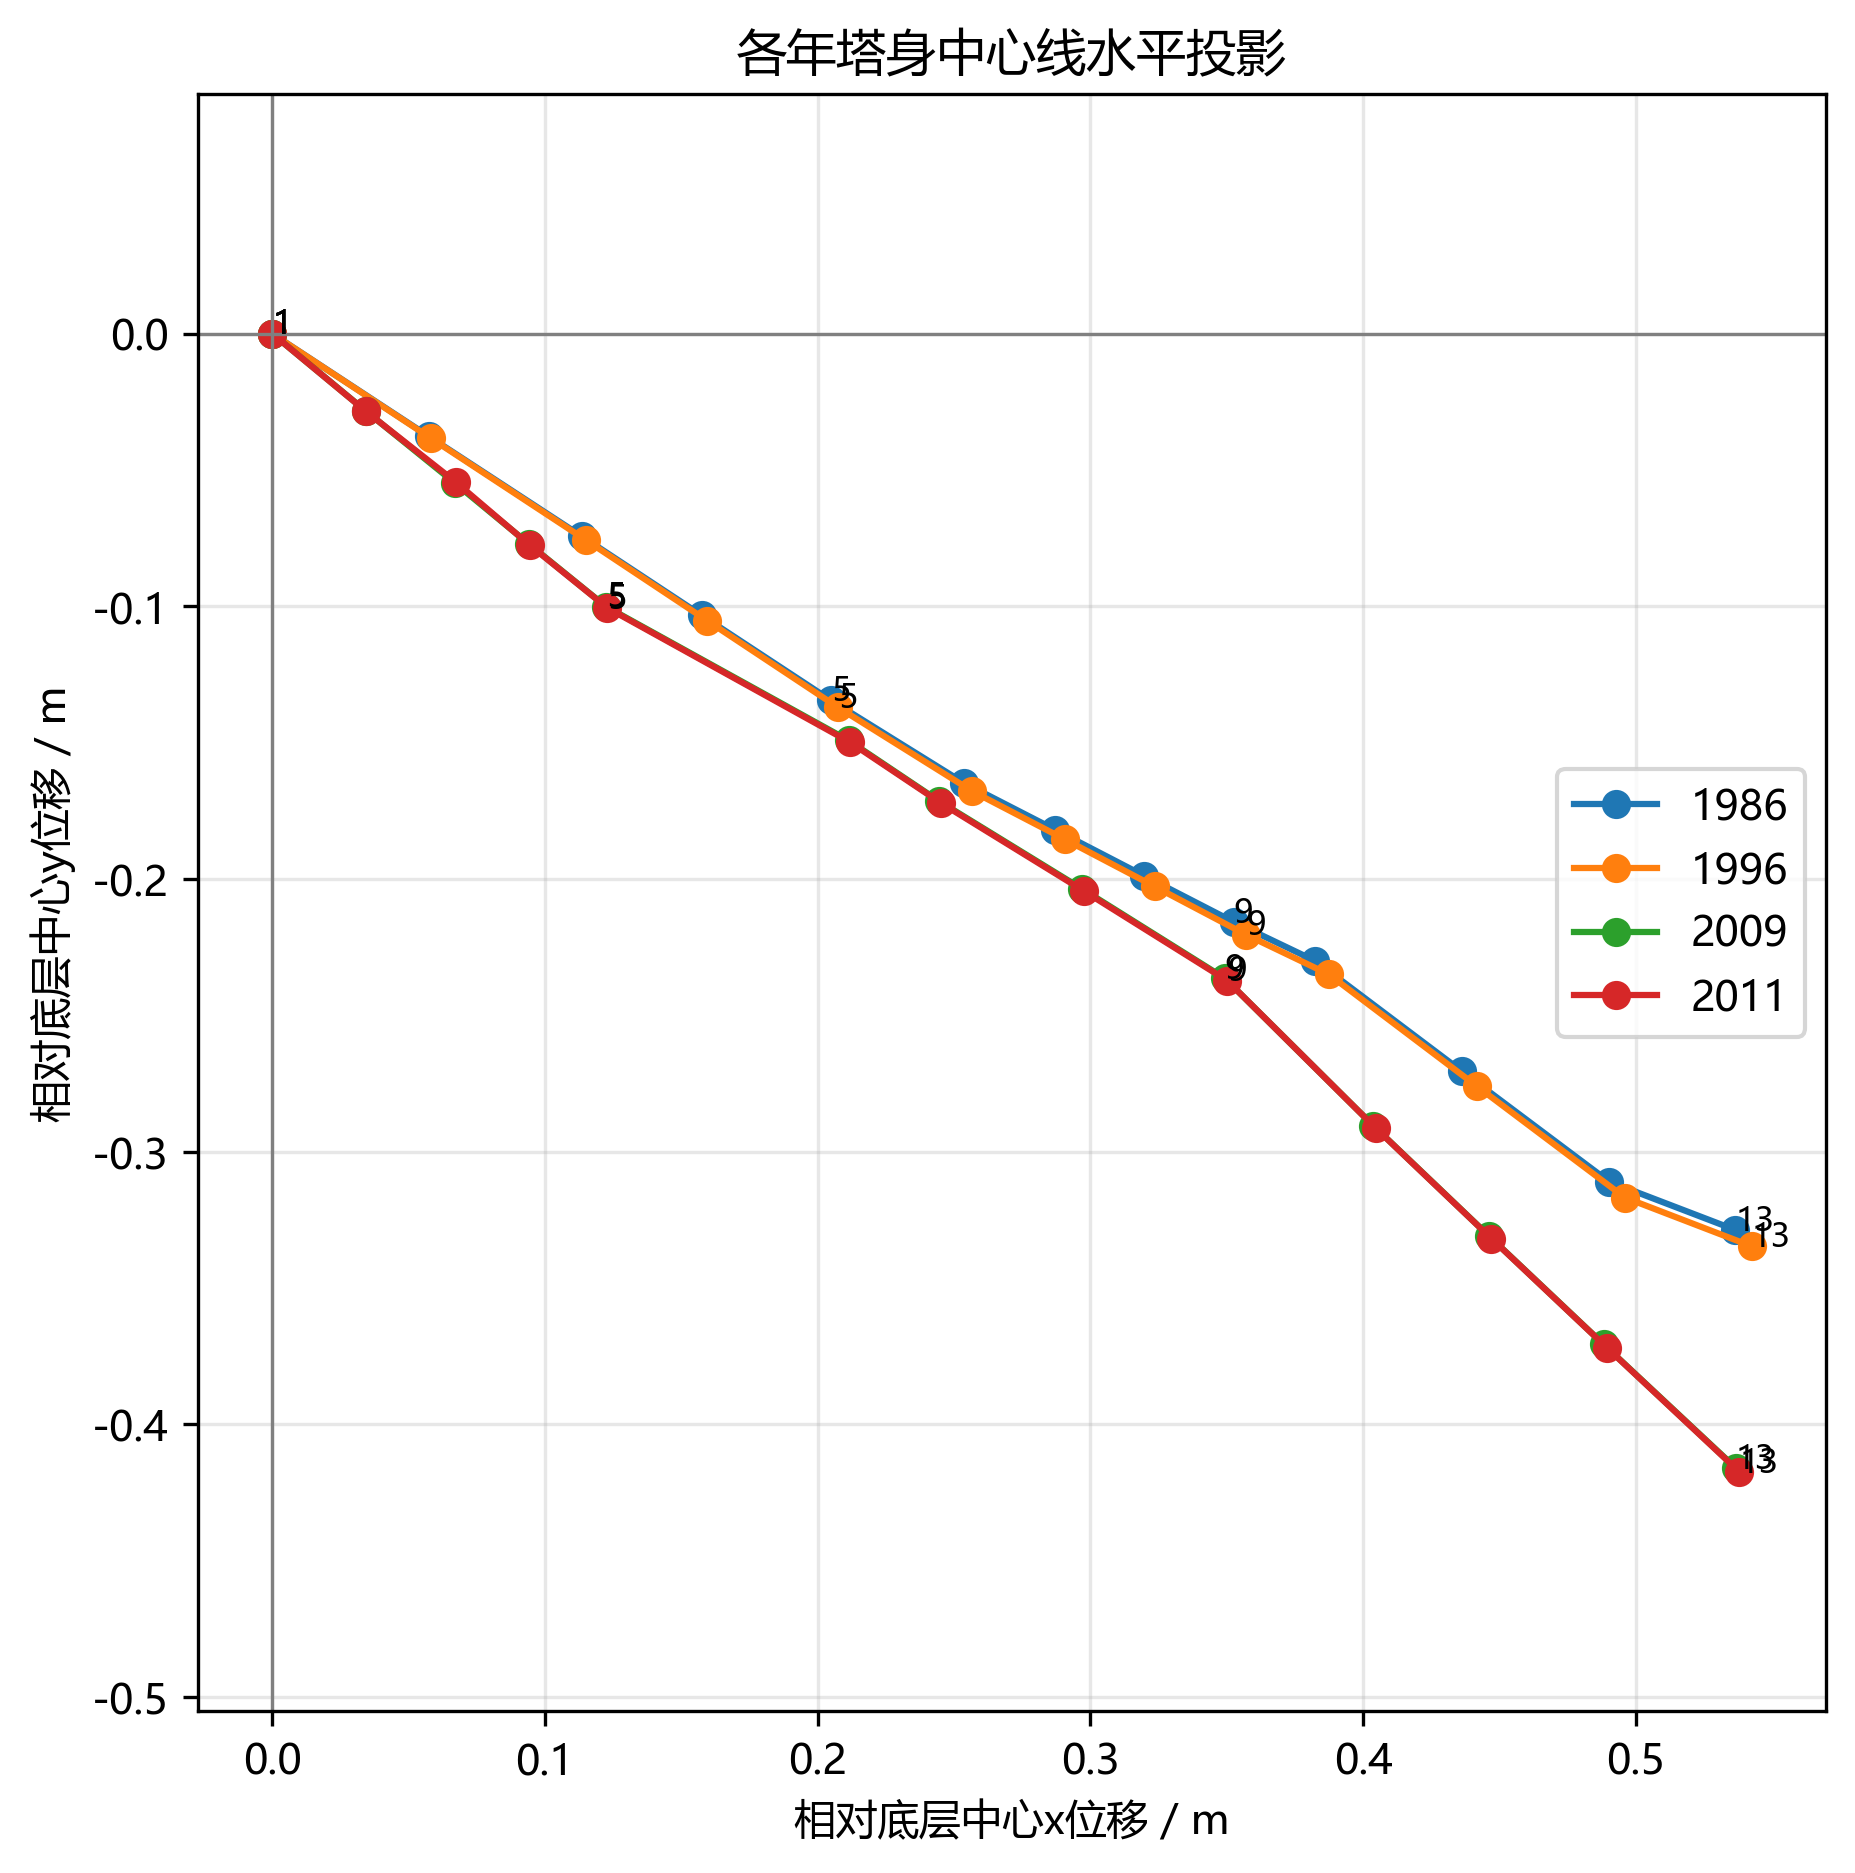
\includegraphics[width=0.72\textwidth]{../quest2/figures/问题2_中心线水平投影.png}
\caption{各年塔身中心线水平投影}
\label{fig:centerline}
\end{figure}

图\ref{fig:centerline}展示了各年度中心线在水平面的投影。四条中心线均从底层原点向$x$正向、$y$负向延伸，说明古塔整体倾斜方向较稳定。2009年和2011年曲线相对1986、1996明显向负$y$方向扩展，表明后期变形主要表现为北向分量增加。由于图中使用相对底层中心坐标，年度坐标基准的整体平移已被剔除。

\begin{figure}[H]
\centering
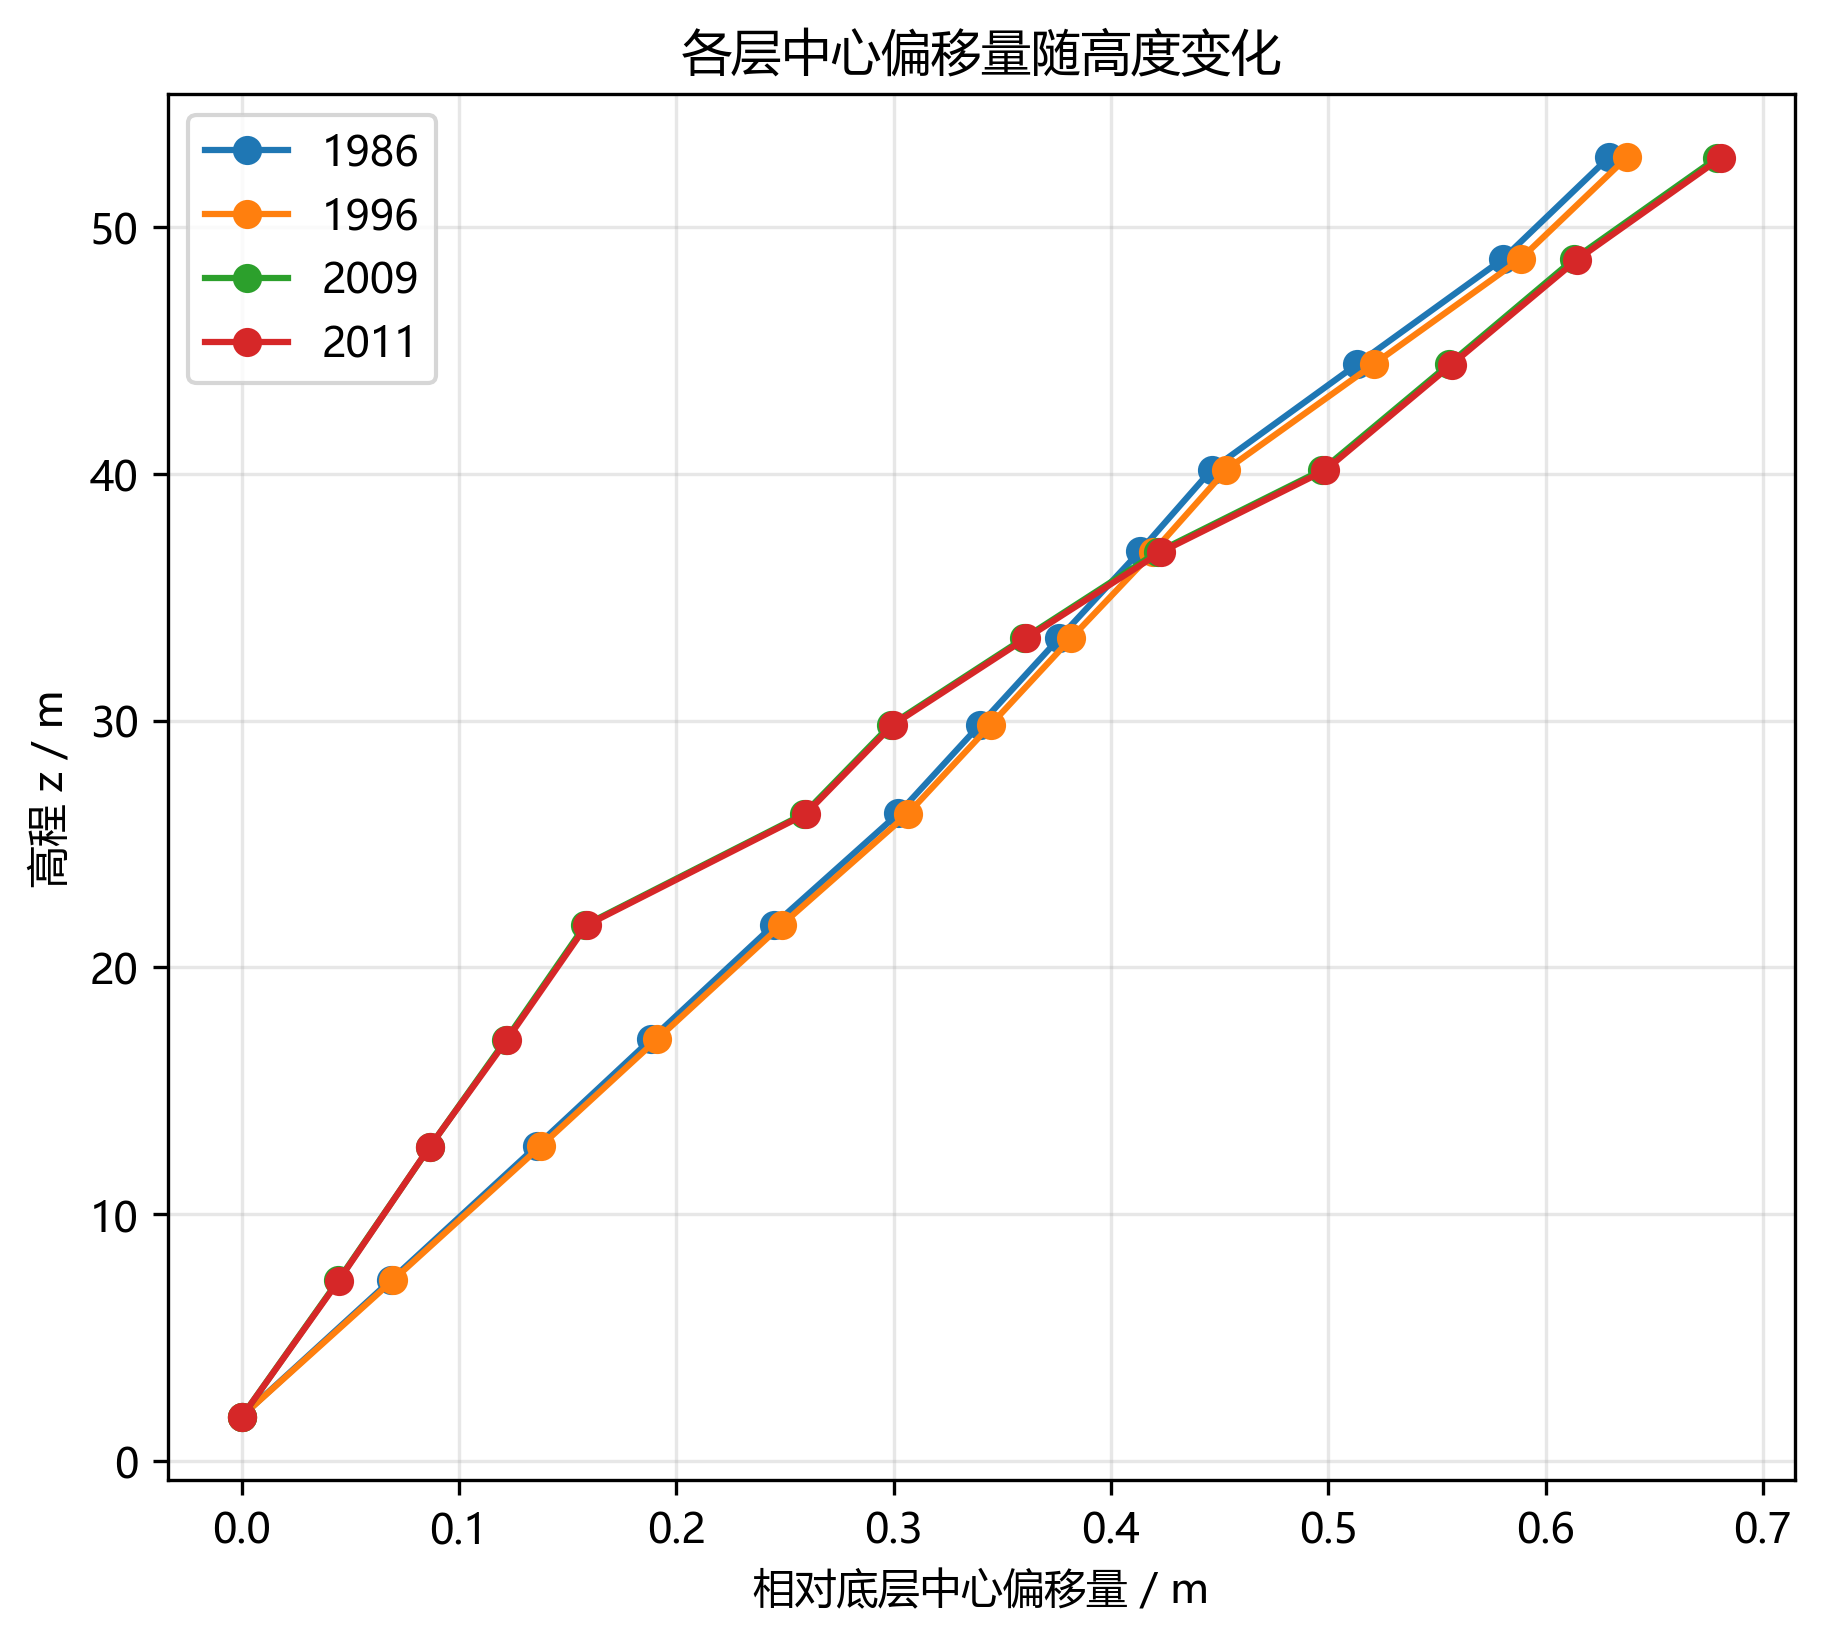
\includegraphics[width=0.74\textwidth]{../quest2/figures/问题2_偏移高度曲线.png}
\caption{各层中心偏移量随高度变化}
\label{fig:offset-height}
\end{figure}

图\ref{fig:offset-height}表明，偏移量总体随高度上升而增加，这符合塔体倾斜的基本特征。第13层偏移从1986年的0.6292 m增加到2011年的0.6808 m，增量约51.6 mm；倾角由0.7062°增加到0.7640°。该量级说明塔体已经存在明确的整体倾斜，应继续监测高层偏移发展。

\begin{table}[H]
\centering
\caption{塔身第13层倾斜指标汇总}
\label{tab:tilt-summary}
\begin{tabular}{rrrrrr}
\toprule
年份 & $\Delta x$ & $\Delta y$ & 偏移量$m$ & 倾角$^\circ$ & 方向角$^\circ$\\
\midrule
1986 & 0.5366 & -0.3287 & 0.6292 & 0.7062 & 328.51\\
1996 & 0.5425 & -0.3347 & 0.6374 & 0.7154 & 328.33\\
2009 & 0.5367 & -0.4160 & 0.6791 & 0.7621 & 322.22\\
2011 & 0.5379 & -0.4173 & 0.6808 & 0.7640 & 322.20\\
\bottomrule
\end{tabular}
\end{table}

\subsubsection{弯曲模型}
若塔身只是整体刚体倾斜，则各层中心应近似落在一条空间直线上。设以相对高度$h=\Delta z$为自变量，中心线的水平坐标满足
\begin{equation}
\Delta x=a_x+b_x h,\quad \Delta y=a_y+b_y h.
\end{equation}
用最小二乘拟合得到最佳直线轴后，定义弯曲残差为
\begin{equation}
b_{jk}=\sqrt{(\Delta x_{jk}-\widehat{\Delta x}_{jk})^2+(\Delta y_{jk}-\widehat{\Delta y}_{jk})^2}.
\end{equation}
该指标越大，说明该层中心偏离整体倾斜直线越明显，弯曲越显著。

\begin{figure}[H]
\centering
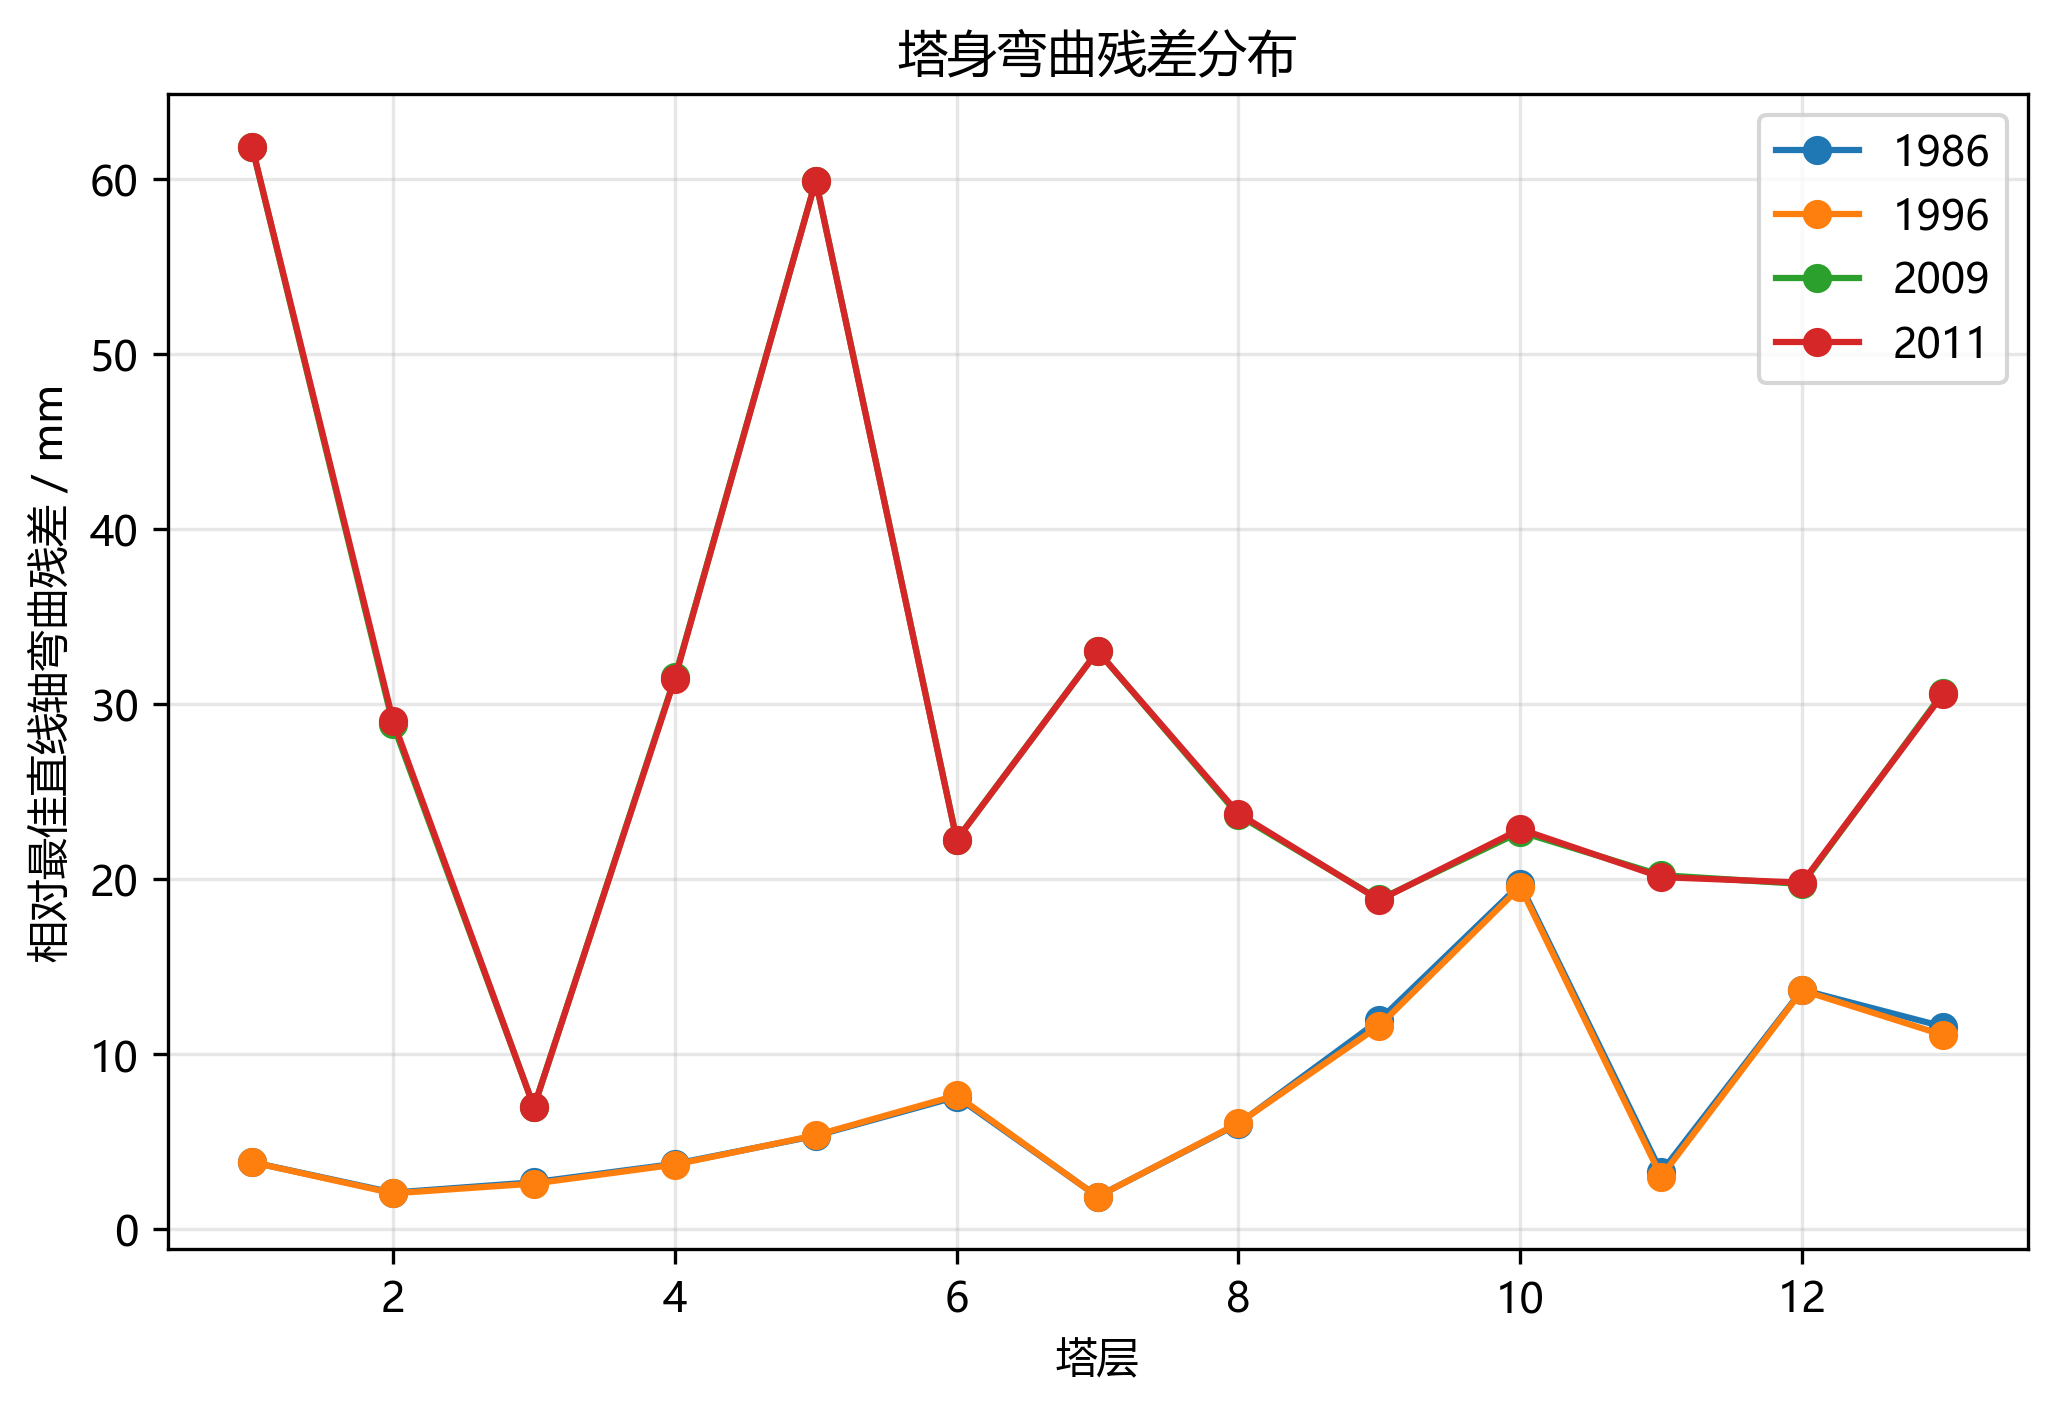
\includegraphics[width=0.78\textwidth]{../quest2/figures/问题2_弯曲残差.png}
\caption{塔身弯曲残差分布}
\label{fig:bending}
\end{figure}

图\ref{fig:bending}显示，1986年和1996年的最大弯曲残差约0.0196 m，弯曲量较小；2009年和2011年最大弯曲残差增至约0.0619 m，平均弯曲残差由约0.0071 m增至约0.0293 m。该结果表明，后期塔身变形不仅是整体倾斜增加，而且中心线形态也发生了更明显的弯曲。弯曲残差在低层和中高层的相对变化，提示塔体可能存在分段刚度或地基变形传递差异。

\begin{table}[H]
\centering
\caption{年度变形综合指标}
\label{tab:def-summary}
\begin{tabular}{rrrrrr}
\toprule
年份 & 顶层偏移$m$ & 顶层倾角$^\circ$ & 方向角$^\circ$ & 最大弯曲$m$ & 平均弯曲$m$\\
\midrule
1986 & 0.6292 & 0.7062 & 328.51 & 0.0197 & 0.0072\\
1996 & 0.6374 & 0.7154 & 328.33 & 0.0195 & 0.0071\\
2009 & 0.6791 & 0.7621 & 322.22 & 0.0618 & 0.0292\\
2011 & 0.6808 & 0.7640 & 322.20 & 0.0619 & 0.0293\\
\bottomrule
\end{tabular}
\end{table}

\subsubsection{扭曲模型}
对于同一年同一层，先以拟合中心为原点，计算第$i$个环向点的极角
\begin{equation}
\gamma_{ijk}=\operatorname{atan2}(y_{ijk}-y_{jk}^c,x_{ijk}-x_{jk}^c).
\end{equation}
由于测点编号代表相对固定的环向位置，本文以同层1号点经编号修正后的方向角作为截面方向，并与底层截面方向相减，得到相对扭转角$\varphi_{jk}$。为避免角度跨越360°产生跳变，差值统一映射到$[-180^\circ,180^\circ]$区间。

\begin{figure}[H]
\centering
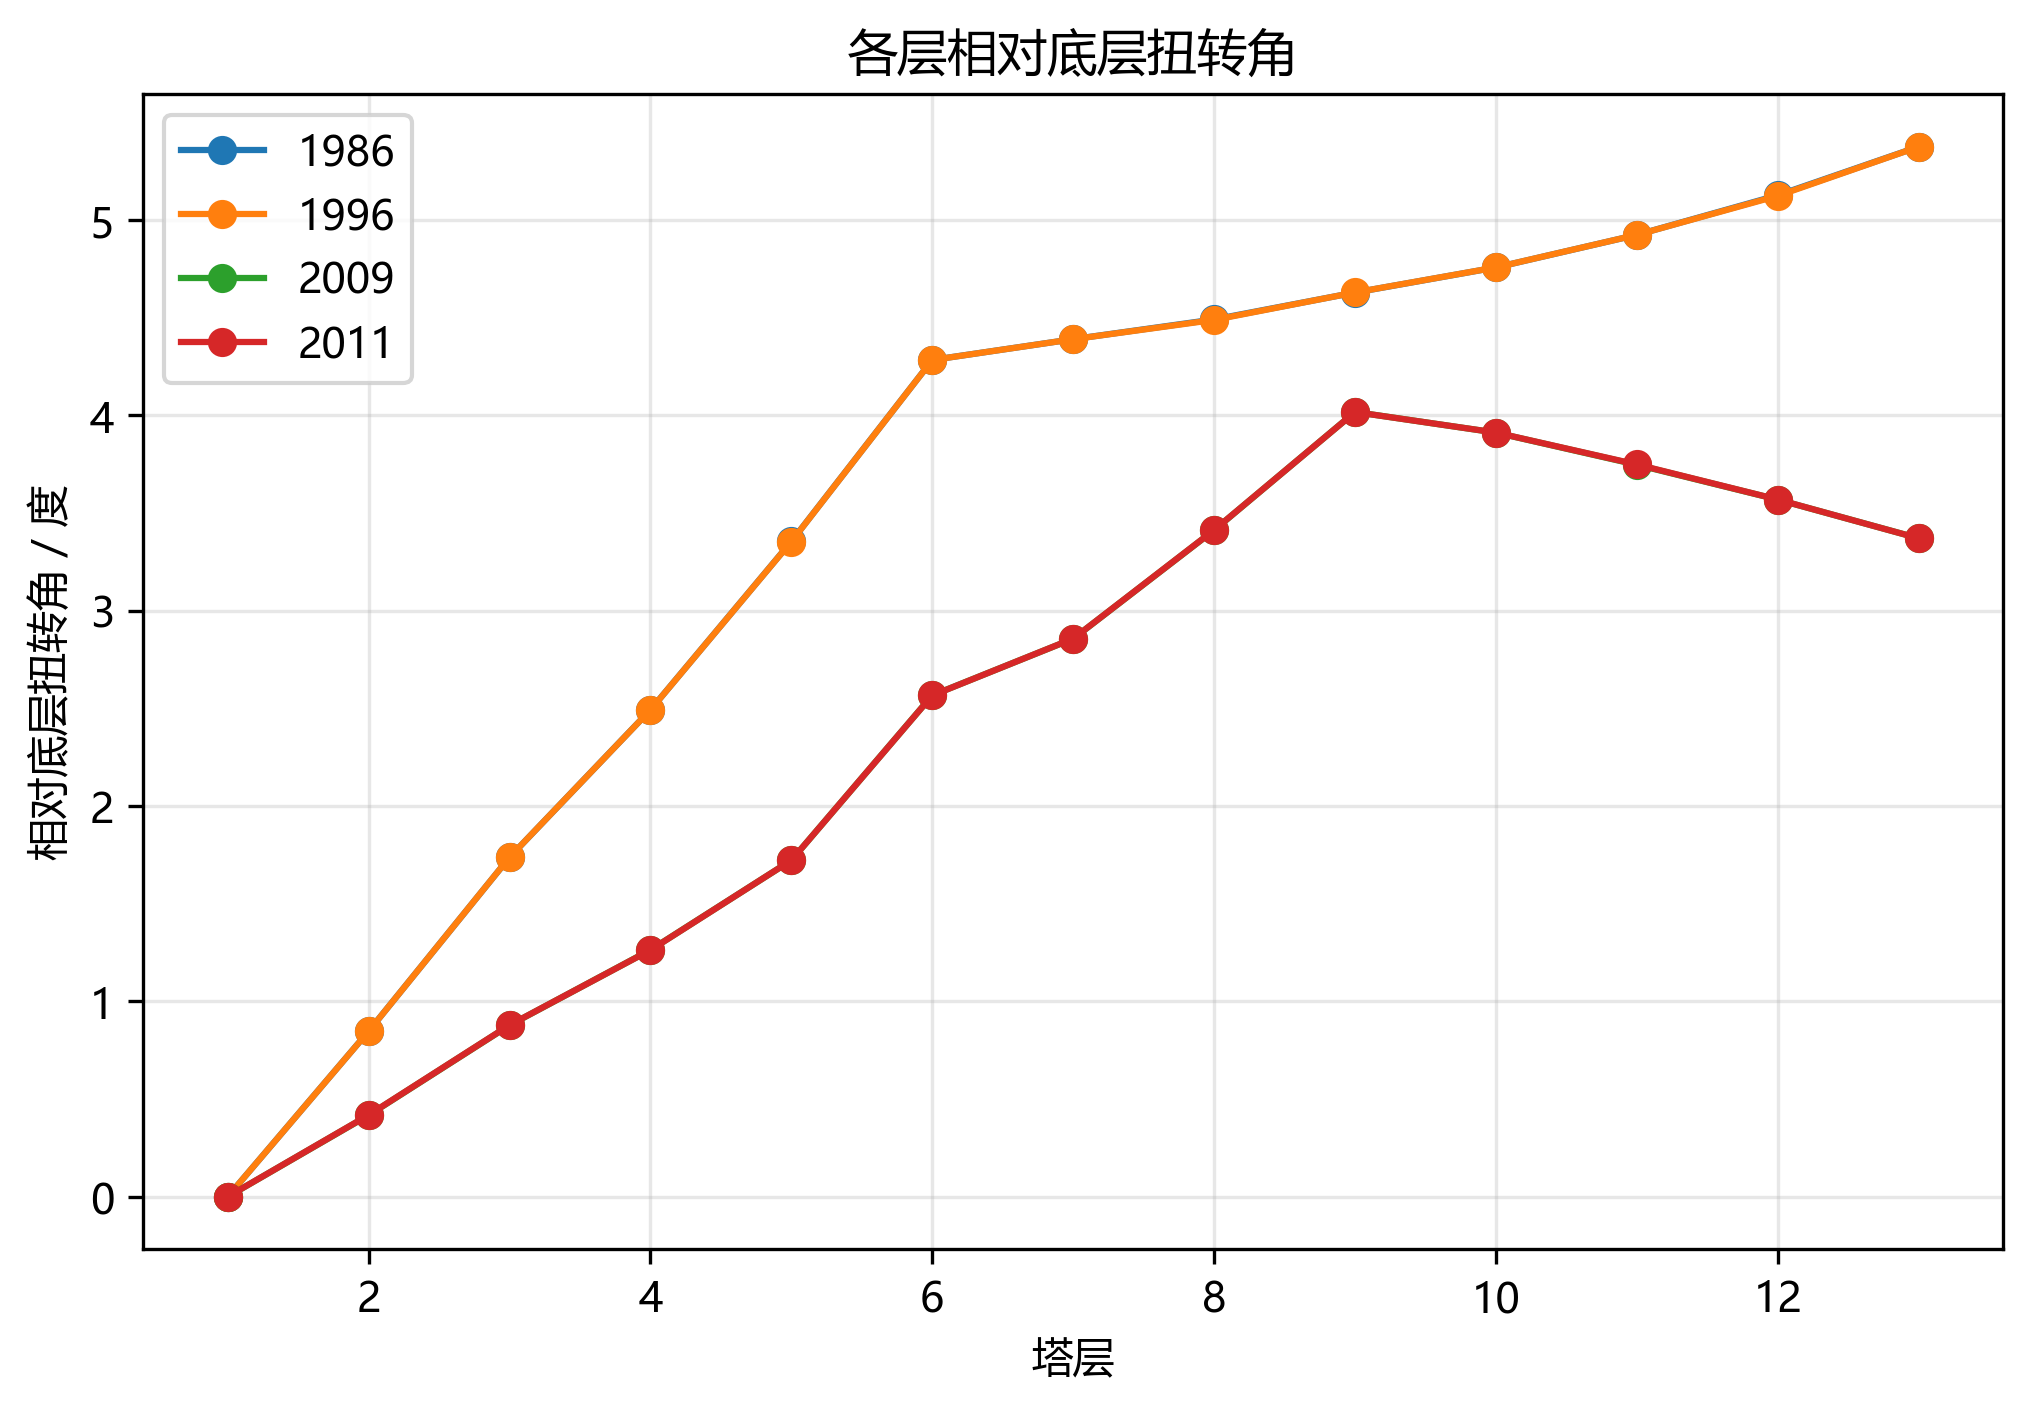
\includegraphics[width=0.78\textwidth]{../quest2/figures/问题2_扭转角.png}
\caption{各层相对底层扭转角}
\label{fig:twist}
\end{figure}

图\ref{fig:twist}表明，各年扭转角随高度存在缓慢变化，但整体幅度不大。1986年和1996年最大相对扭转约5.37°，2009年和2011年最大相对扭转约4.02°。与倾斜偏移和弯曲残差相比，扭曲更像是局部截面方向差异或测点布设方向变化的叠加结果，因此本文将其判定为“可观测但不是主导”的变形类型。实际保护中仍建议保留固定标志点并提高环向观测一致性，以便区分真实扭转与测点编号误差。

\subsection{问题三：变形趋势分析}
\subsubsection{趋势模型建立}
设$t_j=\mathrm{year}_j-1986$，对某一层的偏移量或分量建立线性模型
\begin{equation}
y_{jk}=\beta_{0k}+\beta_{1k}t_j+\varepsilon_{jk}.
\end{equation}
其中$y_{jk}$可取$\Delta x_{jk}$、$\Delta y_{jk}$或$d_{jk}$，$\beta_{1k}$表示年均变化率。模型用最小二乘估计，拟合优度用
\begin{equation}
R^2=1-\frac{\sum_j(y_{jk}-\hat{y}_{jk})^2}{\sum_j(y_{jk}-\bar{y}_k)^2}
\end{equation}
评价。

\subsubsection{趋势结果与预测}
对第13层偏移量的趋势拟合显示，年均增长率为0.00225 m/年，即约2.25 mm/年，$R^2=0.9454$。进一步分解分量可知，$x$向年变化率约$-0.027$ mm/年且$R^2=0.0131$，几乎无稳定趋势；$y$向年变化率约$-3.99$ mm/年且$R^2=0.9059$，说明塔顶偏移发展主要来自$y$负方向分量增加。

\begin{figure}[H]
\centering
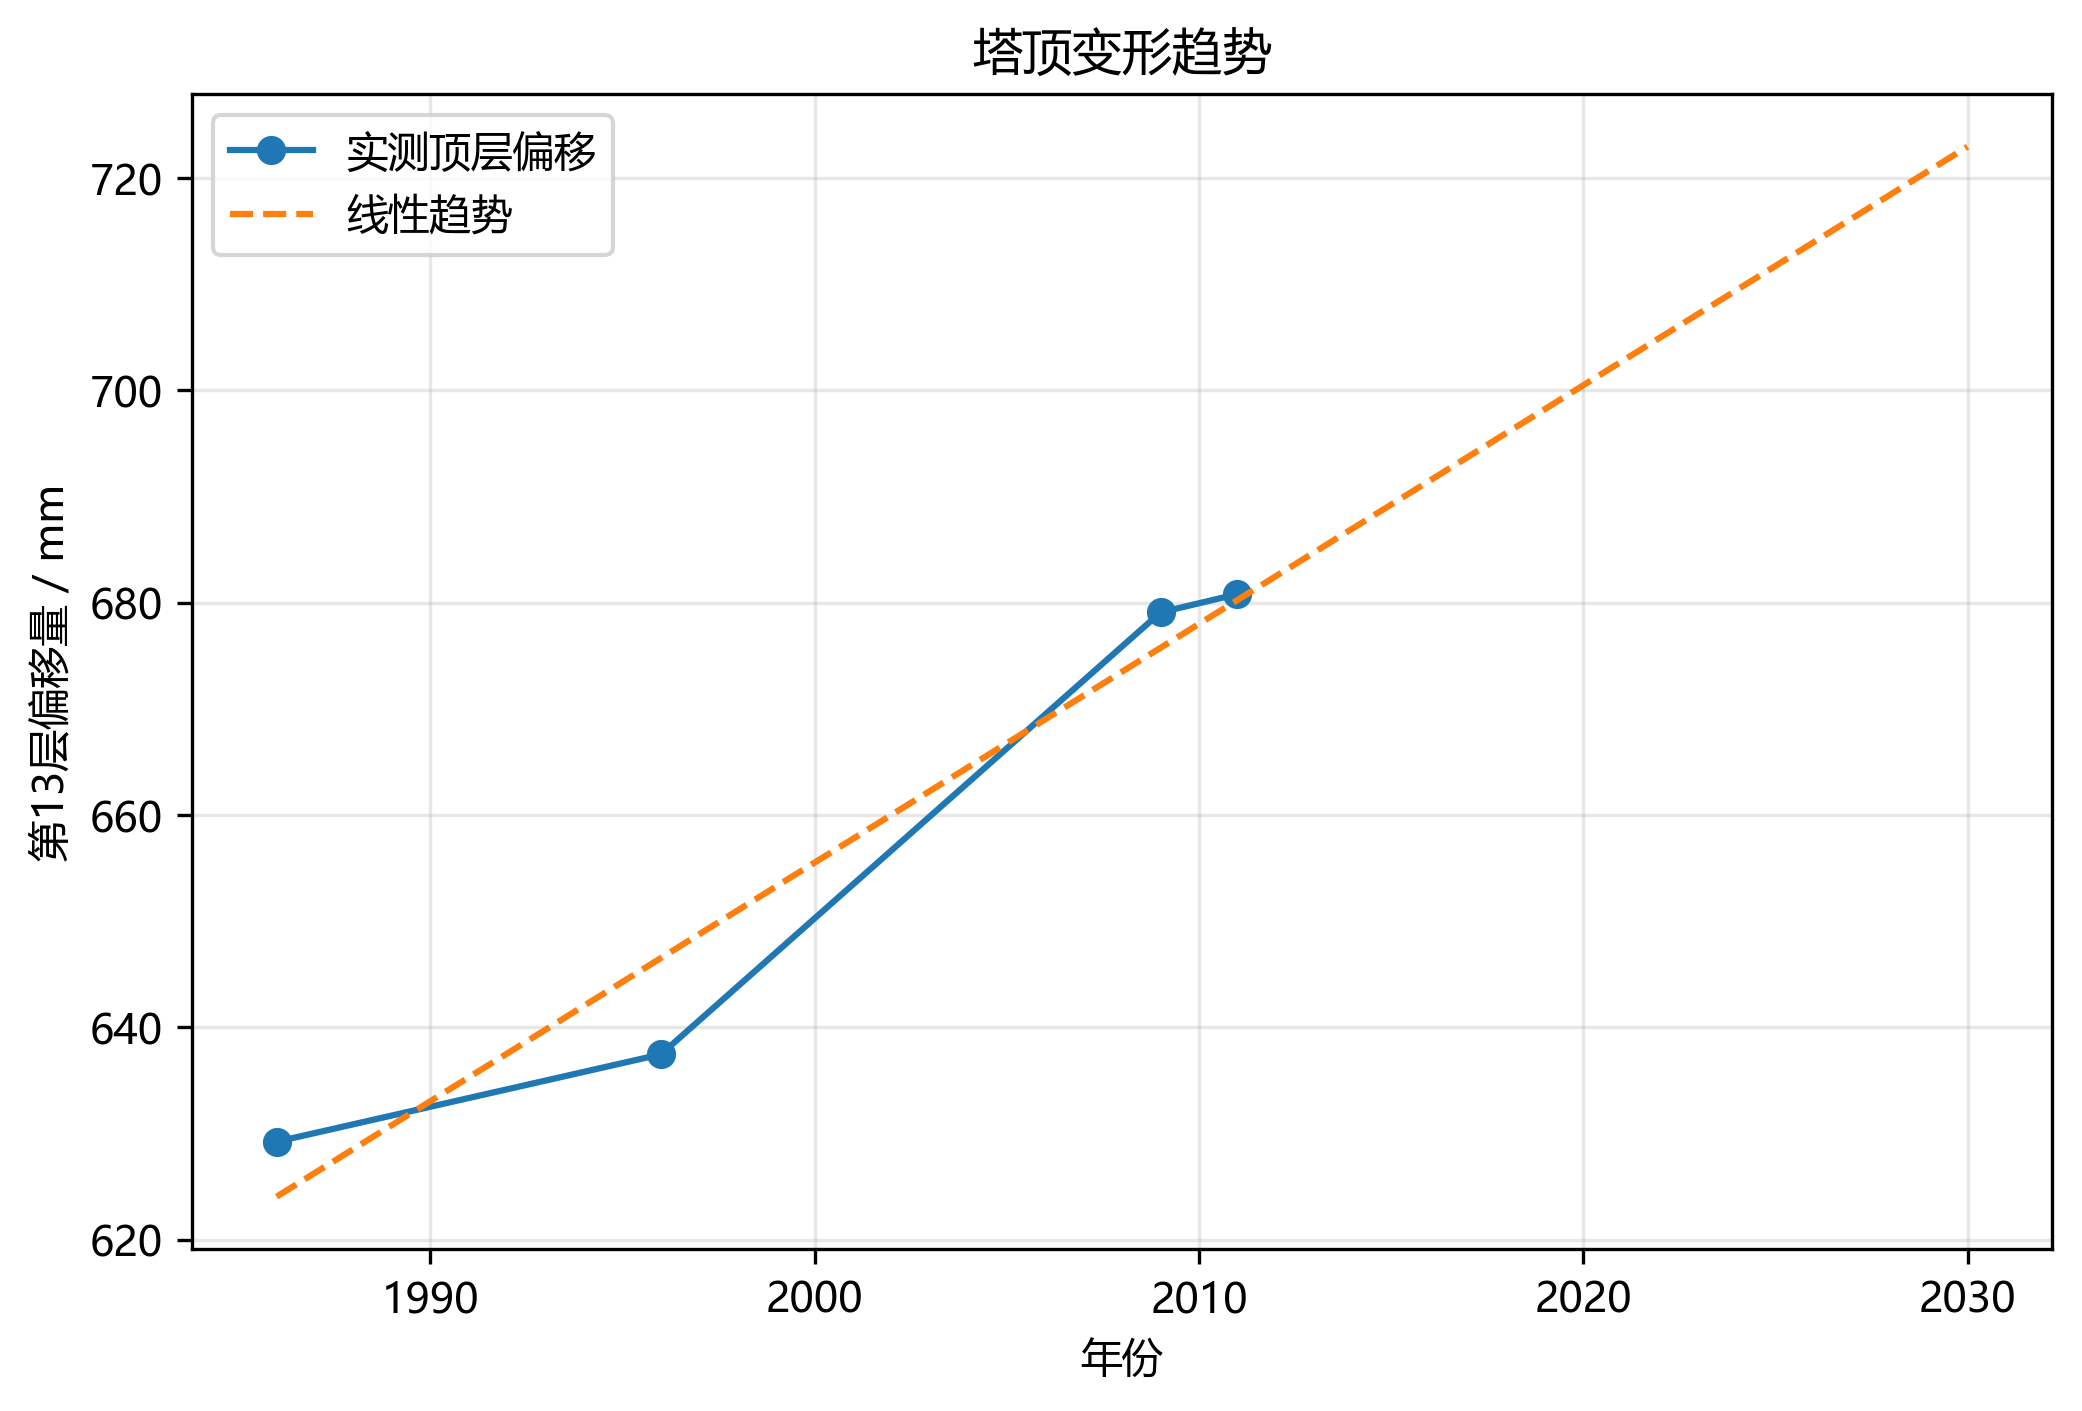
\includegraphics[width=0.78\textwidth]{../quest3/figures/问题3_塔顶偏移趋势.png}
\caption{第13层偏移量趋势拟合与预测}
\label{fig:trend}
\end{figure}

图\ref{fig:trend}给出第13层偏移量的实测值和线性趋势线。1986--1996增长较慢，1996--2009增长较明显，2009--2011增速再次趋缓。由于观测点较少，本文不对这种阶段性变化作复杂非线性解释，而采用线性模型给出保守的平均趋势。预测结果见表\ref{tab:trend-pred}。

\begin{table}[H]
\centering
\caption{第13层变形趋势预测}
\label{tab:trend-pred}
\begin{tabular}{rrrr}
\toprule
年份 & 预测$\Delta x$/m & 预测$\Delta y$/m & 预测偏移量/m\\
\midrule
2021 & 0.5379 & -0.4559 & 0.7051\\
2030 & 0.5376 & -0.4917 & 0.7286\\
\bottomrule
\end{tabular}
\end{table}

由表\ref{tab:trend-pred}可见，若按1986--2011平均趋势继续发展，2021年第13层偏移约0.7051 m，2030年约0.7286 m；方向角将由2011年的322.20°缓慢转向约317.55°。这意味着未来风险并非来自东西向偏移快速增长，而主要来自北向偏移分量持续增加。考虑到文物建筑安全评价通常更关注变化速率和异常突变，建议后续监测重点跟踪第9--13层中心点的$y$向变化率。

\section{模型检验、对比与稳健性分析}
\subsection{中心定位方法检验}
圆拟合模型的可行性首先体现在残差量级。全部层位圆拟合RMS中位数为0.0500 m，最大RMS为0.0774 m，相对层半径2.8--5.4 m占比较小。若采用均值中心，在测点完整且均匀时结果与圆心接近；但1986年和1996年第13层缺失5号点时，均值法不能修正缺失造成的环向不均衡，而圆拟合利用圆方程约束仍可稳定估计中心。因此，圆拟合法相对baseline的优势是对测点缺失和局部噪声更稳健。

\subsection{倾斜与弯曲指标一致性检验}
倾斜指标显示第13层偏移从0.6292 m增至0.6808 m；弯曲指标显示最大残差从约0.0197 m增至约0.0619 m。两者方向一致：塔体后期整体偏移增加，同时中心线偏离直线轴的程度也增加。若仅用塔顶偏移评价，会漏掉弯曲残差增大的信息；若仅用弯曲残差评价，又不能说明整体倾斜方向。两类指标互补，增强了变形诊断的完整性。

\subsection{趋势模型稳健性分析}
本文对第13层趋势进行分量检验。偏移量$d$的线性$R^2=0.9454$，说明总体趋势拟合较好；$y$向分量$R^2=0.9059$，说明主要趋势来自负$y$方向；$x$向分量$R^2=0.0131$，说明$x$方向不宜外推解释。该分量检验避免了把总偏移增长误解为任意方向均增长。

为了评价外推风险，本文比较2011到2030的预测增量：偏移量从0.6808 m增至0.7286 m，增量约47.8 mm，约相当于1986--2011总增量51.6 mm的92.6\%。由于预测期19年接近历史观测跨度25年的76\%，外推并非极端远期，但仍明显依赖线性假设。若未来监测发现年变化率明显偏离2--4 mm/年，应重新估计模型。

\subsection{参数敏感性讨论}
本文模型关键参数主要包括中心定位方法、年度基准选择和趋势模型形式。若不采用相对底层中心，而直接比较绝对坐标，则2009和2011年度底层中心的整体坐标变化会混入塔体变形，导致趋势解释偏差；因此年度局部基准是必要处理。若将趋势模型替换为最近两期差分，2009--2011的短期增量很小，会低估长期发展速度；若只看1986--2011端点差分，则与线性回归结果接近但无法评价$R^2$。综合看，本文选择“相对底层坐标+四期线性回归”对小样本趋势问题更稳健。

\section{模型评价、改进与推广}
\subsection{模型优点}
第一，中心定位模型充分利用了塔层截面几何信息。与简单均值相比，最小二乘圆拟合不仅给出中心，还同时给出半径和残差，便于判断某层数据是否异常。该方法对少量缺测点有较强容忍度，适合文物建筑监测中常见的局部不可测情形。

第二，变形分析区分了倾斜、弯曲和扭曲三类现象。很多简单报告只给出塔顶偏移量，但塔身安全状态与中心线形态密切相关。本文通过最佳直线轴残差识别弯曲，通过极角变化识别扭曲，使结论更接近题目“各种变形量”的要求。

第三，模型使用相对底层中心坐标，降低了跨年份测量基准差异的影响。该处理使不同年份的比较更关注塔体内部几何关系，而不是绝对坐标系统的平移变化，符合长期变形监测的数据特点。

\subsection{模型局限}
第一，附件仅有4个观测年份，趋势模型不可避免存在小样本限制。线性回归能给出平均发展速度，但无法识别地震、维修、地基水文变化等突发因素造成的非线性变化。因此，本文预测应理解为基于历史平均趋势的短中期参考，而非确定性预报。

第二，本文假设每层截面近似圆形，而真实古塔可能存在八边形、局部风化、构件变形等非圆截面因素。圆拟合中心仍能作为稳健几何中心，但半径和残差不能完全等同于真实截面变形，需要结合建筑结构图纸进一步解释。

第三，扭曲分析依赖测点编号在不同年份和层位之间的一致性。如果某次测量点号起始方向不同，极角差异中会混入编号或观测布设误差。本文已将扭曲结论表述为辅助诊断，但若要作为结构安全指标，还需现场确认标志点对应关系。

\subsection{改进方向与推广}
后续可从三方面改进。第一，增加观测期数并采用分段线性或状态空间模型，以识别阶段性加速和突变。第二，引入三维激光扫描或摄影测量点云，用椭圆拟合、鲁棒RANSAC圆拟合等方法替代普通最小二乘，提高对局部损伤点的抗干扰能力。第三，结合地基沉降、风荷载和结构材料参数建立力学解释模型，把几何变形与可能成因联系起来。

本文方法可推广到烟囱、水塔、古建筑塔刹、桥塔等高耸结构的长期几何变形监测。只要每个高度截面有多个环向测点，就可先拟合截面中心，再建立中心线变形指标，实现从测量点数据到结构变形诊断的自动化转换。

\section{结论}
本文完成了2013C“古塔的变形”问题的全过程建模，主要结论如下：
\begin{enumerate}
    \item 各层中心可用最小二乘圆拟合稳定确定。四期数据共得到55组中心结果，圆拟合RMS中位数0.0500 m，最大0.0774 m；完整中心坐标已输出至支撑材料表格。
    \item 古塔存在明确整体倾斜。第13层相对底层中心偏移由1986年的0.6292 m增至2011年的0.6808 m，倾角由0.7062°增至0.7640°，方向角约322°--329°，整体向东偏北方向倾斜。
    \item 塔身存在明显弯曲，且2009年后更突出。最大弯曲残差由约0.0197 m增至约0.0619 m，说明塔体不是单纯刚体倾斜，而是中心线形态也发生变化。
    \item 扭曲变形可观测但不是主导。各年最大相对扭转约4.02°--5.37°，建议作为辅助监测指标，并在后续测量中保证固定点号对应关系。
    \item 变形趋势主要来自$y$负方向分量发展。第13层偏移量年均增加约2.25 mm，$R^2=0.9454$；预测2021年偏移约0.7051 m，2030年约0.7286 m。建议后续重点监测第9--13层中心的北向位移和弯曲残差变化。
\end{enumerate}

\begin{thebibliography}{9}
\bibitem{survey} 武汉大学测绘学院. 工程测量学[M]. 北京: 测绘出版社, 2016.
\bibitem{lsq} 王振杰, 刘经南. 最小二乘原理及其测量数据处理应用[M]. 武汉: 武汉大学出版社, 2018.
\bibitem{struct} 朱伯芳. 结构变形监测与安全评价[M]. 北京: 中国建筑工业出版社, 2015.
\bibitem{circle} Chernov N. Circular and linear regression: fitting circles and lines by least squares[M]. Boca Raton: CRC Press, 2010.
\bibitem{heritage} ICOMOS. Principles for the Analysis, Conservation and Structural Restoration of Architectural Heritage[S]. 2003.
\bibitem{cumcm} 全国大学生数学建模竞赛组委会. 全国大学生数学建模竞赛论文格式规范[EB/OL].
\end{thebibliography}

\newpage
\appendix
\section{支撑材料与复现说明}
\subsection{文件目录}
本题所有产物均位于题目目录下的\texttt{支撑材料/}中，主要包括：
\begin{itemize}
    \item \texttt{papper/论文.tex}与\texttt{papper/论文.pdf}：正式论文源文件和PDF；
    \item \texttt{quest1/codes/main\_modeling.py}：数据读取、圆拟合、变形分析、趋势预测、图表生成和冻结数字的完整脚本；
    \item \texttt{quest2/figures/}与\texttt{quest3/figures/}：论文使用的变形分析和趋势图；
    \item \texttt{tables/}：中心坐标、弯曲残差、扭转角、趋势回归等结果表；
    \item \texttt{results/frozen\_numbers.json}：论文关键数字来源；
    \item \texttt{data/}：原始题面和附件。
\end{itemize}

\subsection{核心代码入口}
核心脚本运行命令如下：
\begin{verbatim}
python quest1/codes/main_modeling.py
\end{verbatim}
脚本将自动读取\texttt{data/附件1.xls}，生成CSV、Excel结果表、PNG图表和冻结数字JSON。全部可视化均使用\texttt{plt.savefig(..., dpi=300, bbox\_inches='tight')}保存，并调用\texttt{plt.close()}关闭图形窗口。

\subsection{关键结果来源}
论文摘要、表\ref{tab:tilt-summary}、表\ref{tab:def-summary}和表\ref{tab:trend-pred}中的关键数字均来自\texttt{results/frozen\_numbers.json}和\texttt{tables/}下最终表格。若重新运行脚本得到不同结果，应先更新冻结数字，再同步修改论文正文和摘要。

\end{document}
